\section{Results}

The data collected, almost 40,000 datapoints, are large and complex and thus will be treated in parts. First a cursory exploration of the data will be presented. Then, each pipeline will be tested against the baseline results, first according to individual features, and then according to each individual pipeline. Following this, each part of the pipeline is examined individually and in combination with the others to identify, analyze, and explain significant differences and interactions. Finally, pipeline features are analyzed in respect to the three question types: single-hop, multi-hop, and adversarial. While two metrics — F1 score (BERTScore) and recall accuracy — were collected, all statistical tests are performed on the former, the latter only being treated in the data exploration section.


%%%%%%%%%%%%%%%%%%%%%%%%%%%%%%%%%%%%%%%%%%%%%%%%%%%%%%

\subsection{Data Exploration}

The test result data, specifically the F1 scores, prove to be eccentric: their distribution is non-normal, heteroscedastic, platykurtic, and highly skewed to the right. Despite this, the data do seem to preserve a similar shape, both as a whole and when grouped by feature variant, which is exemplified in Figure \ref{fig:f1_score_distribution_all} below. Thus, non-parametric approaches to analysis were necessary, namely Mann-Whitley U tests and ART ANOVAs; these will be covered in the following sections. Also, because this abnormal data are not necessarily clustered around the mean, it was more appropriate to look at the medians; this will be the practice for this and future sections.

% Plot
\begin{figure}[p]
\centering
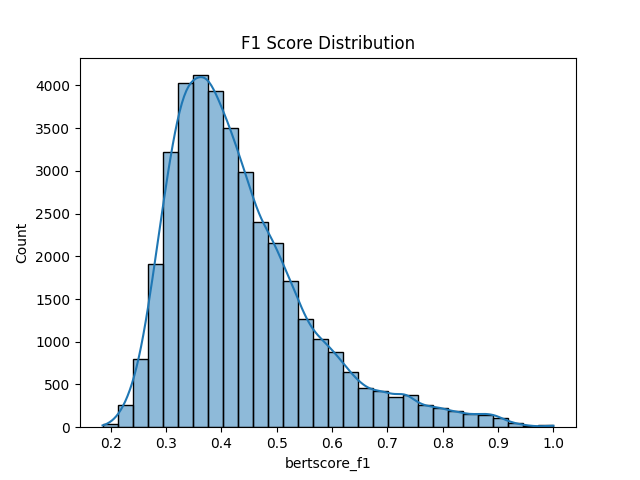
\includegraphics[width=0.75\textwidth]{charts/f1_score_distribution_all.png}
\caption{F1 Score Distribution of All Pipelines}
\label{fig:f1_score_distribution_all}
\end{figure}


\subsubsection{F1 Score}

Looking at the median of each tested pipeline in Table \ref{tab:basic_statistics_table}, as well as the median of the baseline data, reveals some interesting trends. 

First, baseline F1 score is ranked eighth out of all tests and thus divides the data in two, with seven of the LTM models performing better than the baseline, and seventeen performing worse. This division mostly corresponds memory storage format: all seven better-than-baseline models use knowledge bases, while twelve of the seventeen worse-than-baseline models use knowledge graphs. Thus, it appears that knowledge bases outperform knowledge graphs, and are the only memory-storage format that offers any improvement to having no long-term memory at all. 

Additional observations can be made by looking at the knowledge base and graph models that stand out the most. The best performing knowledge graph model stores observations, retrieves them based on cosine similarity, and thereafter performs reflection; this is interesting, since it so happens that the knowledge base equivalent of this pipeline is the second best performing overall. Of the five knowledge base models that perform worse than the baseline, four of them use topic overlap retrieval, four lack a reflection step, and three store summaries. So then, its seems that pipelines involving observations, cosine similarity, and reflection appear to be some of the strongest performing, while those involving summaries, topic overlap, and no reflection some of the weakest performing.

Looking in terms of memory unit types, models storing observations and turns are more likely to perform worse than the baseline, and this tend is even more pronounced for summaries. Turning to retrieval method, a prominent trend is that the top four performing models all employ cosine similarity, while the bottom three performing models employ topic overlap. Finally, all but two better-than-baseline models have a reflection step. Thus, it appears that observations and turns perform better than summaries, cosine similarity performs better than topic overlap, and reflection performs better than no reflection.


\subsubsection{Recall}

Looking at the average recall, again in Table \ref{tab:basic_statistics_table}, one finds that the best performing models tend to have some of the highest recall: the top four performing models have recalls between 51\% to 54\%. 

However, the absolute highest recalls belong not to these, but to models with the combination of knowledge bases and, interestingly enough, summaries: these can have recalls in the range of 70\% to 76\%, even though such models have much lover median F1 scores than their turn and observation counterparts. This seeming discrepancy can be explained by the relatively small size of knowledge bases that store summaries: since summaries are derived from entire sessions, and there are only 19-35 sessions in a \textsc{LoCoMo} conversation, the knowledge bases constructed from these summaries will only have 19 to 35 memories in total. Combined with the \textit{k}-value of 10 used in retrieval, there is a 33\% to 50\% chance that the correct memory will be retrieved at random, which only increases when taking cosine similarity and topic overlap into account.

Another trend is that knowledge graphs appear to have over lower recall rates than knowledge bases: not one knowledge graph model has a higher recall than a knowledge base model. Indeed, the best knowledge graph model recall (0.292161) is almost ten full points behind the worst knowledge base model recall (0.383856). The reason for this difference is difficult to discern, although it might be related to the issues knowledge graphs have with information loss and retrieval, which will be covered future sections.

% Table
\begin{table}[htbp]
\centering
\scriptsize
\begin{tabular}{llllrr}
\toprule
memory\_storage\_format & memory\_unit\_type & retrieval\_method & reflection & bertscore\_f1 & recall \\
\midrule
knowledge base & turn & cosine similarity & True & 0.453117 & 0.532216 \\
knowledge base & observation & cosine similarity & True & 0.452971 & 0.516694 \\
knowledge base & observation & cosine similarity & False & 0.444574 & 0.516694 \\
knowledge base & turn & cosine similarity & False & 0.437911 & 0.532216 \\
knowledge base & turn & topic overlap & True & 0.430522 & 0.439872 \\
knowledge base & summary & cosine similarity & True & 0.430064 & 0.751187 \\
knowledge base & observation & topic overlap & True & 0.428343 & 0.383856 \\
Baseline & Baseline & Baseline & Baseline & 0.420121 & 0.000000 \\
knowledge base & summary & topic overlap & True & 0.419738 & 0.708246 \\
knowledge graph & observation & cosine similarity & True & 0.412327 & 0.212505 \\
knowledge graph & observation & cosine similarity & False & 0.409076 & 0.212505 \\
knowledge graph & turn & cosine similarity & True & 0.404336 & 0.203542 \\
knowledge graph & observation & topic overlap & True & 0.403828 & 0.164406 \\
knowledge base & turn & topic overlap & False & 0.402905 & 0.439872 \\
knowledge graph & summary & cosine similarity & True & 0.401496 & 0.280427 \\
knowledge base & observation & topic overlap & False & 0.400507 & 0.383856 \\
knowledge graph & turn & topic overlap & True & 0.394122 & 0.153908 \\
knowledge graph & summary & topic overlap & True & 0.391807 & 0.292161 \\
knowledge graph & observation & topic overlap & False & 0.391188 & 0.164406 \\
knowledge graph & summary & cosine similarity & False & 0.390025 & 0.280427 \\
knowledge base & summary & cosine similarity & False & 0.387475 & 0.751187 \\
knowledge graph & turn & cosine similarity & False & 0.387198 & 0.203542 \\
knowledge base & summary & topic overlap & False & 0.385587 & 0.708246 \\
knowledge graph & summary & topic overlap & False & 0.376829 & 0.292161 \\
knowledge graph & turn & topic overlap & False & 0.374681 & 0.153908 \\
\bottomrule
\end{tabular}

\caption{F1 Score and Recall for all RAG Pipelines and Baseline}
\label{tab:basic_statistics_table}
\end{table}


%%%%%%%%%%%%%%%%%%%%%%%%%%%%%%%%%%%%%%%%%%%%%%%%%%%%%%

\subsection{Analysis Against Baseline}

Since the data is abnormally distributed and heteroscedastic, but nonetheless regular in general shape, pairwise testing was done using Mann-Whitney U tests with Holm–Bonferroni correction.

The data were compared against the baseline data in two ways. First, the data were grouped according to each variant of each feature of the pipeline (memory storage format, memory unit type, retrieval method, and reflection). In other words, each variant part of the long-term memory pipeline was compared as a group against the baseline. Next, each individual pipeline was compared against the baseline.


\subsubsection{By Feature Variants}

When grouped by feature variant (Tables \ref{tab:memory_storage_format_against_baseline_table} through \ref{tab:reflection_against_baseline_table}), no group of models proved to perform significantly better than the baseline; indeed, only one group, those with knowledge bases, even had a higher median F1 score than the baseline. All other groups of models are significantly outperformed by the baseline. 

These results seem to imply that all tested long-term memory features are no better — and indeed worse — than simply having the language model make educated guesses. However, these exact features were proven to outperform the baseline in all other papers in the current literature (e.g. \cite{Maharana2024}, \cite{Li2024}). The key difference is that those papers only tested models that use knowledge bases as a memory storage format; it follows that the inclusion of knowledge graph models might be responsible for the present discrepancy. Indeed, this appears to be the case: when rerunning the Mann-Whitney U tests with knowledge graph data excluded (Tables \ref{tab:memory_unit_type_against_baseline_table_no_kg} through \ref{tab:reflection_against_baseline_table_no_kg}), feature variants begin to significantly outperform the baseline, namely cosine-similarity, turns, observations, and reflection. Of these, the presence of reflection appears to result in the most marked difference from the baseline (r = -0.084946). Why reflection might have such a pronounced effect size will be covered later.

% Table
\begin{table}[p]
\centering
\tiny
\begin{tabular}{llrrrrrr}
\toprule
Level 1 & Level 2 & Median 1 & Median 2 & Statistic (U) & Raw p-value & Corrected p-value & Rank-biserial corr. \\
\midrule
knowledge base & none & 0.421058 & 0.420121 & 15051412.500000 & 0.210100 & 0.210100 & -0.019014 \\
knowledge graph & none & 0.394159 & 0.420121 & 12611947.500000 & 0.000000 & 0.000000 & 0.146143 \\
\bottomrule
\end{tabular}

\caption{Memory Storage Format against Baseline}
\label{tab:memory_storage_format_against_baseline_table}
\end{table}

% Table
\begin{table}[p]
\centering
\tiny
\begin{tabular}{llrrrrrr}
\toprule
Level 1 & Level 2 & Median 1 & Median 2 & Statistic (U) & Raw p-value & Corrected p-value & Rank-biserial corr. \\
\midrule
observation & none & 0.416780 & 0.420121 & 9744138.500000 & 0.499076 & 0.499076 & 0.010450 \\
turn & none & 0.406920 & 0.420121 & 9308817.000000 & 0.000407 & 0.000814 & 0.054659 \\
summary & none & 0.397231 & 0.420121 & 8610404.500000 & 0.000000 & 0.000000 & 0.125585 \\
\bottomrule
\end{tabular}

\caption{Memory Unit Type against Baseline}
\label{tab:memory_unit_type_against_baseline_table}
\end{table}

% Table
\begin{table}[p]
\centering
\tiny
\begin{tabular}{llrrrrrr}
\toprule
Level 1 & Level 2 & Median 1 & Median 2 & Statistic (U) & Raw p-value & Corrected p-value & Rank-biserial corr. \\
\midrule
cosine similarity & none & 0.414514 & 0.420121 & 14458323.500000 & 0.163500 & 0.163500 & 0.021140 \\
topic overlap & none & 0.398672 & 0.420121 & 13205036.500000 & 0.000000 & 0.000000 & 0.105990 \\
\bottomrule
\end{tabular}

\caption{Retrieval Method against Baseline}
\label{tab:retrieval_method_against_baseline_table}
\end{table}

% Table
\begin{table}[p]
\centering
\tiny
\begin{tabular}{llrrrrrr}
\toprule
Level 1 & Level 2 & Median 1 & Median 2 & Statistic (U) & Raw p-value & Corrected p-value & Rank-biserial corr. \\
\midrule
True & none & 0.416798 & 0.420121 & 14572633.000000 & 0.377083 & 0.377083 & 0.013401 \\
False & none & 0.395878 & 0.420121 & 13090727.000000 & 0.000000 & 0.000000 & 0.113729 \\
\bottomrule
\end{tabular}

\caption{Reflection against Baseline}
\label{tab:reflection_against_baseline_table}
\end{table}

% Table
\begin{table}[p]
\centering
\tiny
\begin{tabular}{llrrrrrr}
\toprule
Level 1 & Level 2 & Median 1 & Median 2 & Statistic (U) & Raw p-value & Corrected p-value & Rank-biserial corr. \\
\midrule
observation & none & 0.432982 & 0.420121 & 5268068.500000 & 0.000018 & 0.000053 & -0.069980 \\
turn & none & 0.431144 & 0.420121 & 5238188.500000 & 0.000088 & 0.000176 & -0.063911 \\
summary & none & 0.405148 & 0.420121 & 4545155.500000 & 0.000002 & 0.000010 & 0.076849 \\
\bottomrule
\end{tabular}

\caption{Memory Unit Type against Baseline (knowledge graphs excluded)}
\label{tab:memory_unit_type_against_baseline_table_no_kg}
\end{table}

% Table
\begin{table}[p]
\centering
\tiny
\begin{tabular}{llrrrrrr}
\toprule
Level 1 & Level 2 & Median 1 & Median 2 & Statistic (U) & Raw p-value & Corrected p-value & Rank-biserial corr. \\
\midrule
cosine similarity & none & 0.432617 & 0.420121 & 7869343.000000 & 0.000031 & 0.000063 & -0.065544 \\
topic overlap & none & 0.411232 & 0.420121 & 7182069.500000 & 0.080519 & 0.080519 & 0.027516 \\
\bottomrule
\end{tabular}

\caption{Retrieval Method against Baseline (knowledge graphs excluded)}
\label{tab:retrieval_method_against_baseline_table_no_kg}
\end{table}

% Table
\begin{table}[p]
\centering
\tiny
\begin{tabular}{llrrrrrr}
\toprule
Level 1 & Level 2 & Median 1 & Median 2 & Statistic (U) & Raw p-value & Corrected p-value & Rank-biserial corr. \\
\midrule
True & none & 0.435632 & 0.420121 & 8012634.500000 & 0.000000 & 0.000000 & -0.084946 \\
False & none & 0.406260 & 0.420121 & 7038778.000000 & 0.002882 & 0.002882 & 0.046918 \\
\bottomrule
\end{tabular}

\caption{Reflection against Baseline (knowledge graphs excluded)}
\label{tab:reflection_against_baseline_table_no_kg}
\end{table}


\subsubsection{By Pipeline}

Looking at each long-term memory pipeline that was tested individually (Table \ref{tab:individual_pipelines_against_baseline_table}, presented in landscape), we find which of the trends discussed in the data exploration subsection are statistically significant. 

The most striking observation is that all but one knowledge graph pipeline perform significantly worse than the baseline; only the top-performing knowledge graph model, which involves observations, cosine similarity, and reflection, is not significantly worse, and only barely so (p-value = 0.061958).

Next, of the seven pipelines that performed better than the baseline, six do so significantly. These six all use knowledge bases, and store either turns or observations. Of these, the top four performing models are all highly significant, and retrieve memories using cosine similarity. The other two are only slightly significant (p-values = 0.020339, 0.010427), and retrieve memories using topic overlap. The non-significant pipeline, unlike the others, stores summaries; also, while non-significant, it is only barely so (p-value = 0.061958). 

Meanwhile, of the seventeen pipelines that performed worse than the baseline, fourteen do so significantly. The sole exceptions are knowledge base models which both use topic overlap, and the best performing knowledge graph model, which was previously mentioned. Given that twenty-four pipelines were tested in total, this means that the majority of long-term memory pipelines tested are significantly worse than having no long-term memory at all. Common among these are a reliance on knowledge graphs, and among those which use knowledge bases, the use of topic overlap, summaries, and a lack of reflection.

% Table
\begin{sidewaystable}[htbp]
\centering
\scriptsize
\begin{tabular}{llrrrrrr}
\toprule
Level 1 & Level 2 & Median 1 & Median 2 & Statistic (U) & Raw p-value & Corrected p-value & Rank-biserial corr. \\
\midrule
knowledge base, turn, cosine similarity, True & none & 0.453117 & 0.420121 & 1420395.500000 & 0.000000 & 0.000000 & -0.153967 \\
knowledge base, observation, cosine similarity, True & none & 0.452971 & 0.420121 & 1436346.500000 & 0.000000 & 0.000000 & -0.166926 \\
knowledge base, observation, cosine similarity, False & none & 0.444574 & 0.420121 & 1368087.000000 & 0.000000 & 0.000001 & -0.111470 \\
knowledge base, turn, cosine similarity, False & none & 0.437911 & 0.420121 & 1343150.500000 & 0.000010 & 0.000087 & -0.091211 \\
knowledge base, turn, topic overlap, True & none & 0.430522 & 0.420121 & 1303783.500000 & 0.004068 & 0.020339 & -0.059228 \\
knowledge base, summary, cosine similarity, True & none & 0.430064 & 0.420121 & 1292310.000000 & 0.015490 & 0.061958 & -0.049907 \\
knowledge base, observation, topic overlap, True & none & 0.428343 & 0.420121 & 1312472.000000 & 0.001303 & 0.010427 & -0.066287 \\
knowledge base, summary, topic overlap, True & none & 0.419738 & 0.420121 & 1247327.000000 & 0.516930 & 0.516930 & -0.013362 \\
knowledge graph, observation, cosine similarity, True & none & 0.412327 & 0.420121 & 1170665.000000 & 0.017650 & 0.061958 & 0.048921 \\
knowledge graph, observation, cosine similarity, False & none & 0.409076 & 0.420121 & 1154985.500000 & 0.002783 & 0.016697 & 0.061659 \\
knowledge graph, turn, cosine similarity, True & none & 0.404336 & 0.420121 & 1108128.500000 & 0.000001 & 0.000014 & 0.099727 \\
knowledge graph, observation, topic overlap, True & none & 0.403828 & 0.420121 & 1110816.000000 & 0.000002 & 0.000022 & 0.097544 \\
knowledge base, turn, topic overlap, False & none & 0.402905 & 0.420121 & 1170859.000000 & 0.018018 & 0.061958 & 0.048763 \\
knowledge graph, summary, cosine similarity, True & none & 0.401496 & 0.420121 & 1097167.500000 & 0.000000 & 0.000002 & 0.108632 \\
knowledge base, observation, topic overlap, False & none & 0.400507 & 0.420121 & 1151163.000000 & 0.001681 & 0.011770 & 0.064765 \\
knowledge graph, turn, topic overlap, True & none & 0.394122 & 0.420121 & 1049563.500000 & 0.000000 & 0.000000 & 0.147307 \\
knowledge graph, summary, topic overlap, True & none & 0.391807 & 0.420121 & 1023658.000000 & 0.000000 & 0.000000 & 0.168353 \\
knowledge graph, observation, topic overlap, False & none & 0.391188 & 0.420121 & 1039603.500000 & 0.000000 & 0.000000 & 0.155399 \\
knowledge graph, summary, cosine similarity, False & none & 0.390025 & 0.420121 & 1040190.500000 & 0.000000 & 0.000000 & 0.154922 \\
knowledge base, summary, cosine similarity, False & none & 0.387475 & 0.420121 & 1009053.500000 & 0.000000 & 0.000000 & 0.180218 \\
knowledge graph, turn, cosine similarity, False & none & 0.387198 & 0.420121 & 1017843.500000 & 0.000000 & 0.000000 & 0.173077 \\
knowledge base, summary, topic overlap, False & none & 0.385587 & 0.420121 & 996465.000000 & 0.000000 & 0.000000 & 0.190445 \\
knowledge graph, summary, topic overlap, False & none & 0.376829 & 0.420121 & 904233.000000 & 0.000000 & 0.000000 & 0.265377 \\
knowledge graph, turn, topic overlap, False & none & 0.374681 & 0.420121 & 895093.000000 & 0.000000 & 0.000000 & 0.272803 \\
\bottomrule
\end{tabular}

\caption{Individual Pipelines against Baseline}
\label{tab:individual_pipelines_against_baseline_table}
\end{sidewaystable}


\subsubsection{Examining the Performance of Knowledge Graphs}

Given these baseline tests, a major observation can be made: knowledge graph models not only fail to outperform a baseline which relies on educated guesses, but somehow significantly performs worse than it. This would imply, then, that knowledge graphs are not merely incapable of providing models with the correct memories, but actively prevent the model from answering correctly, even if it could have guessed the correct answer. While explanations can be found for why knowledge graphs perform worse than knowledge bases, as will be seen later, why they should be worse than the baseline is not immediately obvious. 

One might speculate, however, that knowledge graphs actively misinform the chatbot due to the way it understands the task of remembering. While the chatbot might be free to make educated guesses when no memories are available, when they \textit{are} available the chatbot is asked to make use of them in formulating its answer. This might shift the chatbot's priorities, so that it cares more about using the retrieved memories to make an answer, than whether that answer makes sense given the context. And, given the poor recall that knowledge graphs exhibit, this means that the memories the chatbot tries to make an answer from are much more likely to lack the correct answer. In other words, when the chatbot has access to memories, it becomes in a sense "overconfident" in those memories, and trusts them more than its own intuition, thus providing a confident misinformed answer instead of a tentative educated guess. However, this is only speculation, and a deeper investigation of this phenomenon would go beyond the scope of this thesis.


%%%%%%%%%%%%%%%%%%%%%%%%%%%%%%%%%%%%%%%%%%%%%%%%%%%%%%

\subsection{Tests Within Features}

Having finished testing features and pipelines against the baseline, it comes time to test the variants of each feature against the others. Like with the baseline tests, pairwise testing was carried out using Mann-Whitney U tests with Holm–Bonferroni correction. Below each feature is considered in turn.

% Table
\begin{table}[p]
\centering
\tiny
\begin{tabular}{llrrrrrr}
\toprule
Level 1 & Level 2 & Median 1 & Median 2 & Statistic (U) & Raw p-value & Corrected p-value & Rank-biserial corr. \\
\midrule
knowledge base & knowledge graph & 0.421058 & 0.394159 & 202029113.500000 & 0.000000 & 0.000000 & -0.139818 \\
\bottomrule
\end{tabular}

\caption{Memory Storage Format Variants Comparison}
\label{tab:memory_storage_format_variants_comparison_table}
\end{table}

% Table
\begin{table}[p]
\centering
\tiny
\begin{tabular}{llrrrrrr}
\toprule
Level 1 & Level 2 & Median 1 & Median 2 & Statistic (U) & Raw p-value & Corrected p-value & Rank-biserial corr. \\
\midrule
observation & summary & 0.416780 & 0.397231 & 86739698.500000 & 0.000000 & 0.000000 & -0.101088 \\
turn & observation & 0.406920 & 0.416780 & 75799831.500000 & 0.000000 & 0.000000 & 0.037784 \\
turn & summary & 0.406920 & 0.397231 & 83599832.500000 & 0.000000 & 0.000000 & -0.061230 \\
\bottomrule
\end{tabular}

\caption{Memory Unit Type Variants Comparison}
\label{tab:memory_unit_type_variants_comparison_table}
\end{table}

% Table
\begin{table}[p]
\centering
\tiny
\begin{tabular}{llrrrrrr}
\toprule
Level 1 & Level 2 & Median 1 & Median 2 & Statistic (U) & Raw p-value & Corrected p-value & Rank-biserial corr. \\
\midrule
cosine similarity & topic overlap & 0.414514 & 0.398672 & 190299585.500000 & 0.000000 & 0.000000 & -0.073642 \\
\bottomrule
\end{tabular}

\caption{Retrieval Method Variants Comparison}
\label{tab:retrieval_method_variants_comparison_table}
\end{table}

% Table
\begin{table}[p]
\centering
\tiny
\begin{tabular}{llrrrrrr}
\toprule
Level 1 & Level 2 & Median 1 & Median 2 & Statistic (U) & Raw p-value & Corrected p-value & Rank-biserial corr. \\
\midrule
True & False & 0.416798 & 0.395878 & 192449006.500000 & 0.000000 & 0.000000 & -0.085769 \\
\bottomrule
\end{tabular}

\caption{Reflection Variants Comparison}
\label{tab:reflection_variants_comparison_table}
\end{table}

% Table
\begin{table}[p]
\centering
\tiny
\begin{tabular}{llrrrrrr}
\toprule
Level 1 & Level 2 & Median 1 & Median 2 & Statistic (U) & Raw p-value & Corrected p-value & Rank-biserial corr. \\
\midrule
observation & summary & 0.432982 & 0.405148 & 22250600.500000 & 0.000000 & 0.000000 & -0.129811 \\
turn & observation & 0.431144 & 0.432982 & 19610502.000000 & 0.680501 & 0.680501 & 0.004244 \\
turn & summary & 0.431144 & 0.405148 & 22124596.000000 & 0.000000 & 0.000000 & -0.123413 \\
\bottomrule
\end{tabular}

\caption{Memory Unit Type Variants Comparison (knowledge graphs excluded)}
\label{tab:memory_unit_type_variants_comparison_table_no_kg}
\end{table}

% Table
\begin{table}[p]
\centering
\tiny
\begin{tabular}{llrrrrrr}
\toprule
Level 1 & Level 2 & Median 1 & Median 2 & Statistic (U) & Raw p-value & Corrected p-value & Rank-biserial corr. \\
\midrule
cosine similarity & topic overlap & 0.432617 & 0.411232 & 47667499.500000 & 0.000000 & 0.000000 & -0.075732 \\
\bottomrule
\end{tabular}

\caption{Retrieval Method Variants Comparison (knowledge graphs excluded)}
\label{tab:retrieval_method_variants_comparison_table_no_kg}
\end{table}

% Table
\begin{table}[p]
\centering
\tiny
\begin{tabular}{llrrrrrr}
\toprule
Level 1 & Level 2 & Median 1 & Median 2 & Statistic (U) & Raw p-value & Corrected p-value & Rank-biserial corr. \\
\midrule
True & False & 0.435632 & 0.406260 & 49230046.500000 & 0.000000 & 0.000000 & -0.110994 \\
\bottomrule
\end{tabular}

\caption{Reflection Variants Comparison (knowledge graphs excluded)}
\label{tab:reflection_variants_comparison_table_no_kg}
\end{table}


\subsubsection{Memory Storage Format}

Beginning with memory storage formats, turning to Table \ref{tab:memory_storage_format_variants_comparison_table} we find that knowledge bases perform significantly better than knowledge graphs. This difference is also the greatest in magnitude (r = -0.139818) of those between any feature variants. Given the results presented up until now, which testifies to the stark difference in performance between knowledge base and knowledge graph models, this should hardly be surprising. However, the reasons for this marked difference has up until now not been explored in detail. 

One explanation that has been previously alluded to is that relationship extraction, which is a prerequisite step before uploading text into knowledge graphs, results in information loss. Relationship extraction only selects specific noun, adjective, and verb phrases from a text, and thus anything passed over is missing from the resulting relationship triples. Information and nuances important to answering questions could therefore be excluded from the knowledge graph, meaning relevant memories would be both less informative, and harder to retrieve due to lower cosine similarity and topic overlap scores. For example, take the following question from \textsc{LoCoMo}:

\begin{displayquote}
"What did Caroline research?"
\end{displayquote}

\noindent The answer is "adoption agencies", which can be found in this sentence:

\begin{displayquote}
"Researching adoption agencies — it's been a dream to have a family and give a loving home to kids who need it."
\end{displayquote}

\noindent The relationship triplets extracted from this sentence, however, are the following:

\begin{displayquote}
('it', 's been a dream to have a family and give a loving home to kids who need it', 'N/A')

('it', 's been a dream to have a family', 'N/A')

('it', 's been a dream to give a loving home to kids who need it', 'N/A')

('it', 's been', 'a dream')

('who', 'need it', 'N/A')
\end{displayquote}

\noindent As can be seen, the key piece of information required to answer the question, "researching adoption agencies", didn't match the syntactic criteria that the relationship extractor uses for selecting the source, relationship, and target and thus was omitted. The question becomes unanswerable. Lacking this vital information, these relationship triplets also have an average lower cosine similarity with the question (0.090356088429689) compared to the original text (0.17500635981559753), meaning they are less likely to be retrieved.

The above example hints at another reason for the poor knowledge graph performance: the limitations of the relationship extractor. Of the five relationship triplets extracted from the text above, only one, ('it', 's been', 'a dream'), has both a source and a target. The rest have "N/A" as their target, which is a default result which occurs when the extractor cannot find a valid target. The relationship extractor also has issues with questions:

\begin{displayquote}
"What does Melanie do to destress?"
\end{displayquote}

\noindent becomes

\begin{displayquote}
('what', 'does', 'melanie')
\end{displayquote}

\noindent when the relationship triples are extracted, completely cutting off the main content of the question ("do to relax"), and rendering the question unanswerable. These limitations in the ability to correctly extract the most important relationships from a text, especially when it comes to questions, are certainly a contributing factor to poor performance.

Another flaw inherent to the specific knowledge graph implementation used in this study that can help account for the low F1 scores is that knowledge graph querying is done according to sources and targets, but not according to similar relationships. Since relationships, or edges, contain all the verbal information which defines the relationship between the source and the target, the knowledge graph cannot be explored according to matching verbs. For example, given the sentence "I taught Esperanto", which would result in the triplet ('i', 'taught', 'esperanto'), it is not possible to search for all memories that contain the edge "taught", that is, all memories involving teaching.

This method of querying the knowledge graph was excluded on the grounds that the most frequent edges, such as "is", "like", and "went to", are too semantically light to be useful for querying, and so querying by edges was deemed too impractical to implement. Nonetheless, this omission might also be responsible for the poor performance of knowledge bases.

A final explanation lies not in the structure of the particular knowledge graph used in this study, but in an issue common to all knowledge graphs, again involving how they are queried. Knowledge graphs are queried and explored according to shared sources and targets, i.e. exactly matching noun phrases and predicate adjectives. This technique comes with a major drawback: unless a query contains one of the exact noun or adjective phrases stored in the knowledge graph, it is impossible for the knowledge graph to retrieve the relevant answer. In other words, even if the knowledge graph contains the correct information needed to answer a question, that information might not be retrieved because knowledge graphs have no means of handling paraphrasing and synonyms. Consider the following example. In the \textsc{LoCoMo} dataset, there is this question:\\

"What is Caroline's relationship status?"\\

\noindent When converted to a relationship triple, it looks like this:

\begin{displayquote}
('what', 'is', 'caroline s relationship status')
\end{displayquote}

\noindent The answer to this question, "single", is found in two sentences:

\begin{displayquote}
1) "Their love and help have been so important especially after that tough breakup."

2) "It'll be tough as a single parent, but I'm up for the challenge."
\end{displayquote}

\noindent When converted into relationship triples, the relevant triples are the following:

\begin{displayquote}
1) ('their love and help', 'have been so important especially after', 'that tough breakup')

2) ('it', 'll be tough as', 'a single parent')
\end{displayquote}

\noindent As can be seen, although the phrase "caroline s relationship status" is semantically related to "that tough breakup" and "a single parent", these two memories would never be retrieved from the knowledge graph because they are not exact matches.\\

\noindent \textbf{Note:} Given the drastic difference between knowledge bases and knowledge graphs, both in nature and performance, and the apparent unfeasibility of knowledge graphs, following sections will consider the combined results data, and then the data when excluding knowledge graphs. It is hoped that this will help reveal differences between feature variants that would otherwise be masked by the poor knowledge graph data.


\subsubsection{Memory Unit Type}

Continuing on to memory unit types, in Table \ref{tab:memory_unit_type_variants_comparison_table} we find some interesting results. Considering the data as a whole, we find that models which store observations perform significantly better than those which store turns, while those that store either type of memory unit are significantly better than those which store summaries.

When excluding the knowledge graph data (Table \ref{tab:memory_unit_type_variants_comparison_table_no_kg}) the results are mostly the same, with one key difference: observation models no longer significantly outperform turn models, and indeed to a minor extent the reverse is true: turn models slightly outperform observation models, albeit not significantly.

These results more or less support those of \cite{Maharana2024}: observation models outperform turn models, and both outperform summary models. As for why this pattern exists, there are several possible explanations. Summaries inherently involve the loss of information, and thus are less likely to contain the information needed to answer any particular question. However, this also applies to observations: the number of observations is always lower than the amount of turns in a session, with a general ratio of one observation to every three turns, meaning that information is always lost. And yet, observations are nonetheless either superior or at least on par with turns in terms of F1 scores.

The reason why storing observations produces better results than storing summaries might be a simple matter of prompting: according to the prompts used for generating the observations and summaries found in \textsc{LoCoMo}, the LLM is free to make as many observations from a session transcript as it it sees fit, whereas it demands this same information be condensed into a single summary. The result is that the LLM is free to give each significant piece of information its own separate observation, while for summaries it must make concessions. 

As for why observations can outperform turns, which inherently involve no information loss, the answer might be a matter of information consolidation. Information that would split up between multiple turns in a turn model, including pronouns and other indirect references, would be consolidated into a single observation. In other words, while a turn model would have to retrieve two or three specific turns to get the full context needed to answer a question, an observation model would only need to return one. However, this doesn't explain why observations perform no better than turns when knowledge graph data is excluded. 


\subsubsection{Retrieval Method}


Looking at Tables \ref{tab:retrieval_method_variants_comparison_table} and \ref{tab:retrieval_method_variants_comparison_table_no_kg}, there is a consistent pattern in retrieval methods: cosine similarity performs significantly better than topic overlap. However, this directly contradicts the findings of \cite{Li2024}, despite the fact that the method used in the present study was taken directly from that one. Still, there are two differences between that implementation of topic overlap retrieval and the present. First, \cite{Li2024} used event summaries — short summaries of each event which occurs in the course of a conversation — as memory units, rather than turns, observations, or session summaries. Second, the present model includes the entire noun phrase as topics in addition to the noun, whereas \cite{Li2024} only define topics as nouns. There are no obvious qualities that event summaries have which would favor topic overlap retrieval, and although the the inclusion of noun phrases as topics might decrease topic overlap scores (since the larger the noun phrase, the greater the total amount of topics for a given query or memory), this only occurs when comparing a less specific topic (e.g. "dogs") to a more specific one (e.g. "big blue dogs"), since this design rewards topics with similar levels of specificity; memories are still perfectly capable of being retrieved based on matching nouns alone.
 
While this discrepancy with previous findings remains unexplained, an explanation for the present results can be found. As with knowledge graphs exploration, topic overlap retrieval relies on the exact matching of strings, rendering it blind to paraphrasing and synonyms. This decreases the chances of retrieving a memory which is necessary for answering a question.


\subsubsection{Reflection}

As with retrieval methods, the presence or absence of reflection shows the same results across both datasets (Tables \ref{tab:reflection_variants_comparison_table} and \ref{tab:reflection_variants_comparison_table_no_kg}): reflection produces significantly higher F1 scores than no reflection. This can be explained by looking at the reflections themselves. When a model (knowledge base, turns, cosine similarity) is presented the question

\begin{displayquote}
"What career path has Caroline decided to persue?"
\end{displayquote}

\noindent the retrieval system returns ten memories, of which only three are relevant\footnote{As mentioned in Section 5.4, first- and second-person pronouns have been replaced with the names of the speaker and addressee, respectively.}:

\begin{displayquote}
"Lately, Caroline has been looking into counseling and mental health as a career. Caroline want to help people who have gone through the same things as Caroline."

"Caroline mentor a transgender teen just like Caroline. We has been working on building up confidence and finding positive strategies, and it's really been paying off! We had a great time at the LGBT pride event last month."

"Woah, Caroline, it sounds like Caroline is doing some impressive work. It's inspiring to see Caroline's dedication to helping others. What motivated Caroline to pursue counseling?"
\end{displayquote}

\noindent When all ten memories are fed into the reflection model, the resulting reflection is the following:

\begin{displayquote}
"As I revisit these memories, I see that Caroline has been seeking a career path that aligns with their values of compassion and helping others. Their personal experiences, including mentoring a transgender teen and overcoming similar challenges, have motivated them to pursue counseling and mental health as a career."
\end{displayquote}

\noindent As can bee seen, the reflection step acts as a filter: given a list of 10 potentially relevant memories, and the question they were retrieved to answer, the reflection model attends only to the memories that appear most relevant to the question. This reduces the amount of information fed into the chatbot during the response generation step, which makes it easier for the chatbot to utilize the information to answer the question correctly. In the case where reflection is not used, the unfiltered memories are given directly the chatbot and could act as noise, hindering the chatbot's ability to answer the question correctly.


%%%%%%%%%%%%%%%%%%%%%%%%%%%%%%%%%%%%%%%%%%%%%%%%%%%%%%

\subsection{Tests Between Features}

Now it is time to turn our attention to what might be the most interesting analyses of this thesis, that of interactions between different features in the conversational RAG pipeline. As with the pairwise comparisons, a non-parametric method was utilized, in this case Aligned Rank Transform ANOVA. Alongside this, plots are presented to ascertain which specific variants of each feature are interacting, and the nature of their interaction. When possible, tentative explanations are offered for these interactions, although most of these cannot be considered definitive, and require further research to confirm or deny.


\subsubsection{Memory Storage Format × Memory Unit Type}
\label{memory_storage_format_x_memory_unit_type}

Significant interactions were found between memory storage formats and memory unit types (Table \ref{tab:memory_storage_format_x_memory_unit_type_table}, Figure \ref{fig:interaction_memory_storage_format_x_memory_unit_type}). This makes sense, since there is an inherent, intimate relationship between a storage system, and that which is stored within it. Looking at the plot, we first find that observations and summaries draw slightly closer in distance when used with knowledge graphs, meaning that observations are particularly more effective than summaries when used with knowledge bases, and that knowledge graphs mitigate this effect. Why this is the case is not immediately clear. Looking at the same plot, however, we find that turns react to memory formats in a much more extreme way: in knowledge bases, they are equal in performance to observations, whereas in knowledge graphs they perform much worse, being equal to summaries. 


% Plot
\begin{figure}[p]
\centering
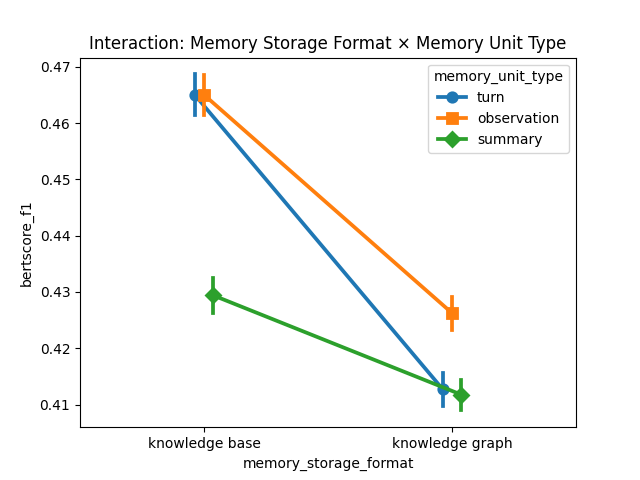
\includegraphics[width=0.75\textwidth]{charts/interaction_memory_storage_format_x_memory_unit_type.png}
\caption{Interactions between Memory Storage Format and Memory Unit Type}
\label{fig:interaction_memory_storage_format_x_memory_unit_type}
\end{figure}

% Plot
\begin{figure}[p]
\centering
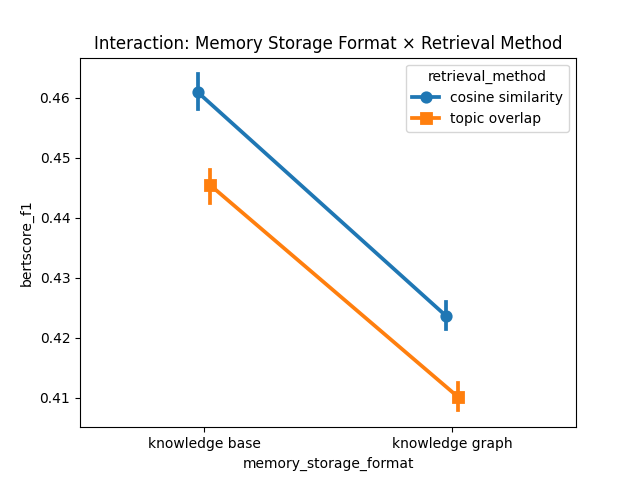
\includegraphics[width=0.75\textwidth]{charts/interaction_memory_storage_format_x_retrieval_method.png}
\caption{Interactions between Memory Storage Format and Retrieval Method}
\label{fig:interaction_memory_storage_format_x_retrieval_method}
\end{figure}


Focusing on this second interaction, one explanation might be that turns, being pure spoken dialogue, are much more grammatically complex than observations, which are simple factual statements, and thus are more difficult for the relationship extractor to successfully parse, leading to worse retrieval and lower F1 scores. This would account for why turns perform much worse than observations when stored in knowledge graphs. 

As for why turn-based models have similar performance to observation-based ones when stored in knowledge bases, it is harder to find an explanation. Earlier it was argued that observations should capture more referential information than turns, in order to explain the significant difference between observations and turns within the data. However, now it can be seen that this difference is only present in the knowledge graph models, and does not hold true for knowledge base ones. Thus we have no choice other than to reject this explanation. 

Instead, we can argue that turns and observations have no real difference in the quality of information they store, leading to similar scores when used in conjunction with knowledge bases.

% Table
\begin{table}[htbp]
\centering
\tiny
\begin{tabular}{lrrrr}
\toprule
 & sum\_sq & df & F & PR(>F) \\
\midrule
C(memory\_storage\_format) & 7764215620.759016 & 1.000000 & 66.021742 & 0.000000 \\
C(memory\_unit\_type) & 2877075893.649273 & 2.000000 & 12.232373 & 0.000005 \\
C(memory\_storage\_format):C(memory\_unit\_type) & 11288676962.470539 & 2.000000 & 47.995712 & 0.000000 \\
Residual & 4427673492927.104492 & 37650.000000 & NaN & NaN \\
\bottomrule
\end{tabular}

\caption{ART ANOVA for Memory Storage Format × Memory Unit Type}
\label{tab:memory_storage_format_x_memory_unit_type_table}
\end{table}


\subsubsection{Memory Storage Format × Retrieval Method}

Only a very slight significant interaction was found between memory storage formats and retrieval methods (Table \ref{tab:memory_storage_format_x_retrieval_method_table}, Figure \ref{fig:interaction_memory_storage_format_x_retrieval_method}); however, the plotted lines for cosine similarity and topic overlap remain more or less parallel between memory storage formats, only ever so slightly narrowing when used with knowledge graphs. Thus, while significant, this interaction is not worth investigating.

% Table
\begin{table}[htbp]
\centering
\tiny
\begin{tabular}{lrrrr}
\toprule
 & sum\_sq & df & F & PR(>F) \\
\midrule
C(memory\_storage\_format) & 8461821515.733070 & 1.000000 & 71.749897 & 0.000000 \\
C(retrieval\_method) & 16801832.237121 & 1.000000 & 0.142467 & 0.705843 \\
C(memory\_storage\_format):C(retrieval\_method) & 637581400.465838 & 1.000000 & 5.406212 & 0.020070 \\
Residual & 4440487255435.046875 & 37652.000000 & NaN & NaN \\
\bottomrule
\end{tabular}

\caption{ART ANOVA for Memory Storage Format × Retrieval Method}
\label{tab:memory_storage_format_x_retrieval_method_table}
\end{table}


\subsubsection{Memory Storage Format × Reflection}

Significant interactions were found between memory storage formats and reflection, with reflection having a much larger effect on F1 scores when used in conjunction with knowledge bases (Table \ref{tab:memory_storage_format_x_reflection_table}, Figure \ref{fig:interaction_memory_storage_format_x_reflection}). One possible explanation for this is the lower recall displayed by knowledge graphs: reflection has been shown to work as a filter which selects which memories out those retrieved are relevant to the question, and since knowledge graphs are much worse at retrieving the correct memories, reflection will be less effective with them.

% Table
\begin{table}[htbp]
\centering
\tiny
\begin{tabular}{lrrrr}
\toprule
 & sum\_sq & df & F & PR(>F) \\
\midrule
C(memory\_storage\_format) & 8507983728.165408 & 1.000000 & 72.217997 & 0.000000 \\
C(reflection) & 103393458.241963 & 1.000000 & 0.877631 & 0.348857 \\
C(memory\_storage\_format):C(reflection) & 5219596560.485344 & 1.000000 & 44.305304 & 0.000000 \\
Residual & 4435772485741.586914 & 37652.000000 & NaN & NaN \\
\bottomrule
\end{tabular}

\caption{ART ANOVA for Memory Storage Format × Reflection}
\label{tab:memory_storage_format_x_reflection_table}
\end{table}


% Plot
\begin{figure}[p]
\centering
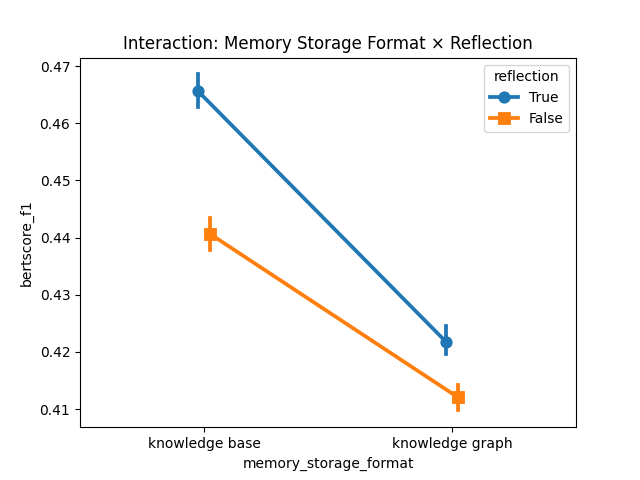
\includegraphics[width=0.75\textwidth]{charts/interaction_memory_storage_format_x_reflection.png}
\caption{Interactions between Memory Storage Format and Reflection}
\label{fig:interaction_memory_storage_format_x_reflection}
\end{figure}

% Plot
\begin{figure}[p]
\centering
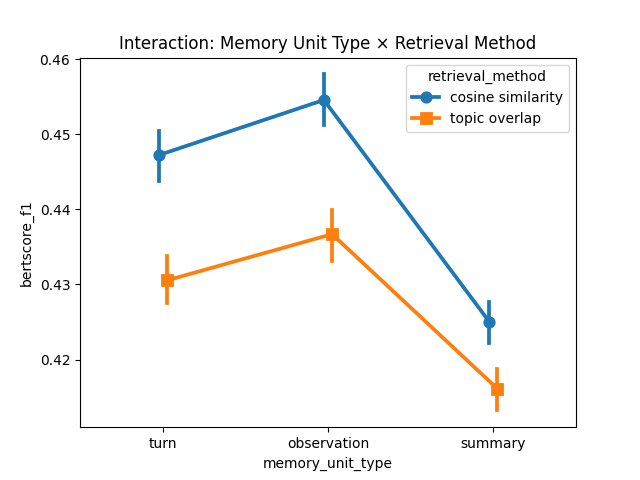
\includegraphics[width=0.75\textwidth]{charts/interaction_memory_unit_type_x_retrieval_method.png}
\caption{Interactions between Memory Unit Type and Retrieval Method}
\label{fig:interaction_memory_unit_type_x_retrieval_method}
\end{figure}


\subsubsection{Memory Unit Type × Retrieval Method}

Memory unit type was shown to have a significant effect on retrieval method, specifically when it comes to summaries (Table \ref{tab:memory_unit_type_x_retrieval_method_table}, Figure \ref{fig:interaction_memory_unit_type_x_retrieval_method}). When summaries are the unit of memory being stored, the difference between cosine similarity and topic overlap is much less than with the other two memory unit types: cosine similarity displays much less of an advantage. This might be the influence of unit length on the effectiveness of cosine similarity. Summaries are on average 650 characters long, whereas turns and observations are only 120 and 90 characters long on average, making summaries roughly six times longer. Having to store six times the information as other embeddings, and in the same number of dimensions, summary embeddings probably suffer from a generally more muted, less distinctive semantic profile, which would lead to less stark differences in cosine similarity scores during retrieval, making the retrieval method less effective.

% Table
\begin{table}[htbp]
\centering
\tiny
\begin{tabular}{lrrrr}
\toprule
 & sum\_sq & df & F & PR(>F) \\
\midrule
C(memory\_unit\_type) & 3874279975.711880 & 2.000000 & 16.411560 & 0.000000 \\
C(retrieval\_method) & 26471068.961635 & 1.000000 & 0.224264 & 0.635812 \\
C(memory\_unit\_type):C(retrieval\_method) & 1681647019.948506 & 2.000000 & 7.123505 & 0.000807 \\
Residual & 4444021063775.873047 & 37650.000000 & NaN & NaN \\
\bottomrule
\end{tabular}

\caption{ART ANOVA for Memory Unit Type × Retrieval Method}
\label{tab:memory_unit_type_x_retrieval_method_table}
\end{table}


\subsubsection{Memory Unit Type × Reflection}

Two significant interactions can be identified between memory unit types and reflection (Table \ref{tab:memory_unit_type_x_reflection_table}, Figure \ref{fig:interaction_memory_unit_type_x_reflection}). First, models storing observations are less effected by a lack of reflection compared to other models. This might be attributed to the previously discussed consolidation and synthesis of information inherent in the creation of observations, which could anticipate the consolidation and synthesis that occurs in reflection: observations have already gone through a form of reflection, and thus the lack of an additional reflection step is less consequential. However, as we have seen in Section \ref{memory_storage_format_x_memory_unit_type}, there is evidence against this hypothesis.

The other significant interaction is that between the lack of reflection and summaries, with the former having a much larger impact on the latter than in other models. As mentioned earlier, summaries are roughly six times larger on average than observations; thus, it might be that chatbots have increased difficulty filtering out the correct information from what is essentially a wall of text, and therefore benefit more from a filtering step like reflection.

% Table
\begin{table}[htbp]
\centering
\tiny
\begin{tabular}{lrrrr}
\toprule
 & sum\_sq & df & F & PR(>F) \\
\midrule
C(memory\_unit\_type) & 4270639549.551753 & 2.000000 & 18.092730 & 0.000000 \\
C(reflection) & 224861641.568090 & 1.000000 & 1.905270 & 0.167498 \\
C(memory\_unit\_type):C(reflection) & 1622205664.088950 & 2.000000 & 6.872537 & 0.001037 \\
Residual & 4443485754737.792969 & 37650.000000 & NaN & NaN \\
\bottomrule
\end{tabular}

\caption{ART ANOVA for Memory Unit Type × Reflection}
\label{tab:memory_unit_type_x_reflection_table}
\end{table}


% Plot
\begin{figure}[p]
\centering
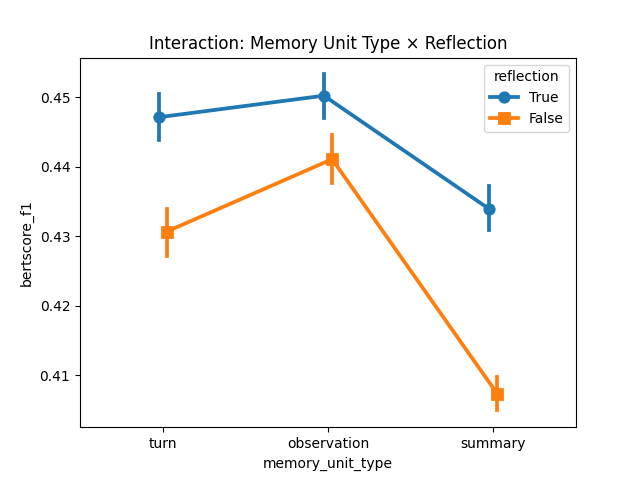
\includegraphics[width=0.75\textwidth]{charts/interaction_memory_unit_type_x_reflection.png}
\caption{Interactions between Memory Unit Type and Reflection}
\label{fig:interaction_memory_unit_type_x_reflection}
\end{figure}

% Plot
\begin{figure}[p]
\centering
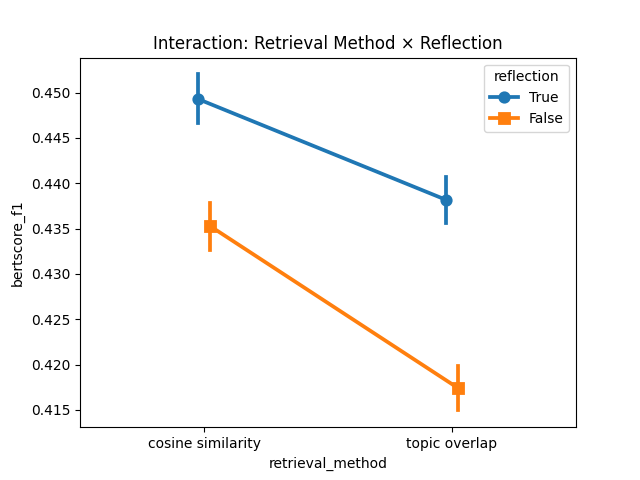
\includegraphics[width=0.75\textwidth]{charts/interaction_retrieval_method_x_reflection.png}
\caption{Interactions between Retrieval Method and Reflection}
\label{fig:interaction_retrieval_method_x_reflection}
\end{figure}


\subsubsection{Retrieval Method × Reflection}

Finally, a slightly significant interaction is found between retrieval method and reflection, with the use of reflection having a slightly larger effect when paired with topic overlap (Table \ref{tab:retrieval_method_x_reflection_table}, Figure \ref{fig:interaction_retrieval_method_x_reflection}). An explanation for why this might be the case, however, doesn't offer itself.

% Table
\begin{table}[htbp]
\centering
\tiny
\begin{tabular}{llrrrr}
\toprule
sum\_sq & df & F & PR(>F) \\
\midrule
60247520.018752 & 1.000000 & 0.509907 & 0.475183 \\
181967688.749743 & 1.000000 & 1.540091 & 0.214612 \\
632206247.051770 & 1.000000 & 5.350703 & 0.020719 \\
4448729038964.180664 & 37652.000000 & NaN & NaN \\
\bottomrule
\end{tabular}

\caption{ART ANOVA for Retrieval Method × Reflection}
\label{tab:retrieval_method_x_reflection_table}
\end{table}


%%%%%%%%%%%%%%%%%%%%%%%%%%%%%%%%%%%%%%%%%%%%%%%%%%%%%%

\subsection{Tests Between Features and Question Types}

The final stage of analysis will now look for interactions between each feature and each of the three question types: single-hop, multi-hop, and antagonistic. Before this, however, we shall look at the major trends that question types exhibit across all features.


\subsubsection{General Trends Exhibited by Question Types}
\label{general_trends_exhibited_by_question_types}

While the interactions between question types and pipeline features can vary widely, as will be seen below, two trends remain constant.

First, single-hop questions always produce the highest F1 scores, followed by multi-hop questions, and then adversarial questions. Single-hop questions leading to better performance than multi-hop questions supports the findings of \cite{Maharana2024}. Since multi-hop questions require a chatbot to retrieve multiple memories, and thus are inherently harder to answer, this pattern is to be expected. 

Second, adversarial questions always produce the lowest, and therefore best, F1 scores for feature variants which have been shown to be the worst performing: knowledge graphs, summaries, topic overlap, and no reflection. This is curious, as it appears unlikely that such poorly performing feature variants would all happen to be predisposed to be better at handling adversarial questions. On the other hand, these results are partially supported by \cite{Maharana2024}, which show that summary models, otherwise the worst performing, actually excel at adversarial questions. Still, it seems more likely that these models are not receiving the correct memories, and responding that they cannot answer the question because they don't know the answer, rather than retrieving the correct information and identifying the question as adversarial. This would result in a bad BERTScore with the adversarial answer, and thus a deceptively low F1 score.


\subsubsection{Memory Storage Format × Question Type}

There is a very significant interaction between the memory storage format and single-hop questions: knowledge base models are much better at answering single-hop questions than the other two types, but for knowledge graph models this performance with single-hop questions is much less pronounced, with F1 scores essentially equal to those of multi-hop questions (Table \ref{tab:memory_storage_format_x_question_type_table}, Figure \ref{fig:interaction_memory_storage_format_x_question_type}). 

Where does this drop off in the ability of knowledge graph models to answer single-hop questions come from? And why do they treat them similarly to multi-hop questions? One possible explanation is that since relationship extraction can convert a single text into multiple discrete triplets of information, the answer to a question which would be contained by a single turn, observation, or summary in a knowledge base would be split into several separate relationship triplets in a knowledge graph. This would mean that single-hop questions would actually become no different than multi-hop questions for knowledge graph models, as multiple relevant triples would need to be returned to answer the question fully. This would explain both why single-hop questions produced a worse performance, and why their performance appears to be the same as multi-hop questions.

% Table
\begin{table}[h]
\centering
\tiny
\begin{tabular}{lrrrr}
\toprule
 & sum\_sq & df & F & PR(>F) \\
\midrule
C(memory\_storage\_format) & 6865893552.409551 & 1.000000 & 58.559864 & 0.000000 \\
C(question\_type) & 7350892592.852382 & 2.000000 & 31.348234 & 0.000000 \\
C(memory\_storage\_format):C(question\_type) & 21085226023.871746 & 2.000000 & 89.918957 & 0.000000 \\
Residual & 4414301445925.313477 & 37650.000000 & NaN & NaN \\
\bottomrule
\end{tabular}

\caption{ART ANOVA for Memory Storage Format × Question Type}
\label{tab:memory_storage_format_x_question_type_table}
\end{table}


\subsubsection{Memory Unit Type × Question Type}
\label{interaction_memory_unit_type_x_question_type}

Two significant interactions can be observed between memory unit types and question types (Table \ref{tab:memory_unit_type_x_question_type_table}, Figure \ref{fig:interaction_memory_unit_type_x_question_type}). 

First, while single- and multi-hop questions produce a constant trend for turns and observations, with the former question type leading to better results than the latter, for summaries single-hop questions lose their advantage, and perform no better than multi-hop questions. This is quite surprising, as this contradicts the results of \cite{Maharana2024} which show that summary models perform more than twice as well on single-hop questions than multi-hop ones. Why this might be the case, is unknown.

Second, unlike the other two question types, which produce higher F1 scores with observation models than with turn models, adversarial questions produce the opposite results: turn models have the higher F1 scores. As theorized in Section \ref{general_trends_exhibited_by_question_types}, it's possible that the F1 scores for adversarial questions don't accurately represent how well a model performed, and that poor memory retrieval could result in low F1 scores. Because of this, an explanation of this trend is not possible.


% Table
\begin{table}[h]
\centering
\tiny
\begin{tabular}{lrrrr}
\toprule
 & sum\_sq & df & F & PR(>F) \\
\midrule
C(memory\_unit\_type) & 3336394640.014003 & 2.000000 & 14.181104 & 0.000001 \\
C(question\_type) & 8531410536.839378 & 2.000000 & 36.262143 & 0.000000 \\
C(memory\_unit\_type):C(question\_type) & 9122442742.766777 & 4.000000 & 19.387141 & 0.000000 \\
Residual & 4428613212876.884766 & 37647.000000 & NaN & NaN \\
\bottomrule
\end{tabular}

\caption{ART ANOVA for Memory Unit Type × Question Type}
\label{tab:memory_unit_type_x_question_type_table}
\end{table}


\subsubsection{Retrieval Method × Question Type}

When looking at retrieval methods and question types, a significant interaction was found: multi-hop questions result in significantly worse F1 scores for topic overlap models (Table \ref{tab:retrieval_method_x_question_type_table}, Figure \ref{fig:interaction_retrieval_method_x_question_type}). More specifically, cosine similarity models handle multi-hop questions nearly as well as single-hop ones, both with much higher F1 scores than adversarial questions, while it was the reverse for topic overlap models, whose F1 scores for multi-hop questions resemble those for adversarial questions. Why this might be the case, however, is not immediately clear.

% Table
\begin{table}[h]
\centering
\tiny
\begin{tabular}{lrrrr}
\toprule
 & sum\_sq & df & F & PR(>F) \\
\midrule
C(retrieval\_method) & 25682262.971798 & 1.000000 & 0.218082 & 0.640508 \\
C(question\_type) & 9272628090.726065 & 2.000000 & 39.369433 & 0.000000 \\
C(retrieval\_method):C(question\_type) & 6478976517.943932 & 2.000000 & 27.508235 & 0.000000 \\
Residual & 4433826172184.858398 & 37650.000000 & NaN & NaN \\
\bottomrule
\end{tabular}

\caption{ART ANOVA for Retrieval Method × Question Type}
\label{tab:retrieval_method_x_question_type_table}
\end{table}


\subsubsection{Reflection × Question Type}

A final interaction was found between reflection and question type, with multi-hop questions performing significantly worse with models lacking reflection (Table \ref{tab:reflection_x_question_type_table}, Figure \ref{fig:interaction_reflection_x_question_type}). This is to be expected, since the reflection step involves synthesizing information from retrieved memories, which is important for multi-hop questions. When a model lacks a reflection step and is tasked with answering a multi-hop question, then, the correct answer is not fed to the model already pieced together, meaning it would have to do so during the more complex chatbot generation step, which would lead to more errors and a lower F1 score.

% Table
\begin{table}[htbp]
\centering
\tiny
\begin{tabular}{lrrrr}
\toprule
 & sum\_sq & df & F & PR(>F) \\
\midrule
C(reflection) & 216668286.657645 & 1.000000 & 1.838047 & 0.175188 \\
C(question\_type) & 9477839064.107950 & 2.000000 & 40.201340 & 0.000000 \\
C(reflection):C(question\_type) & 1740505254.709300 & 2.000000 & 7.382552 & 0.000623 \\
Residual & 4438168445741.525391 & 37650.000000 & NaN & NaN \\
\bottomrule
\end{tabular}

\caption{ART ANOVA for Reflection × Question Type}
\label{tab:reflection_x_question_type_table}
\end{table}


% Plot
\begin{figure}[htbp]
\centering
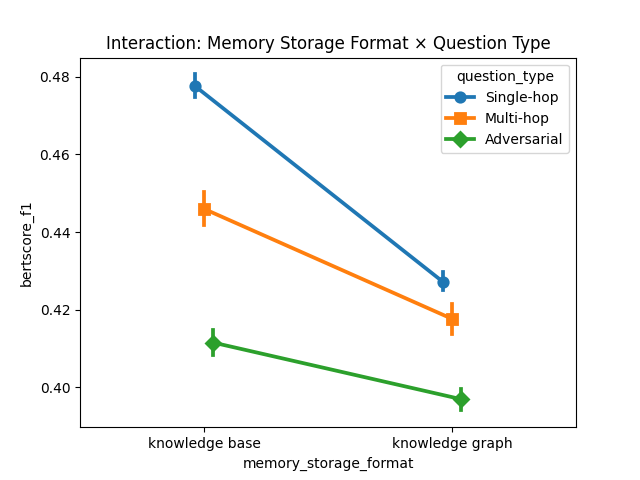
\includegraphics[width=0.75\textwidth]{charts/interaction_memory_storage_format_x_question_type.png}
\caption{Interactions between Memory Storage Format and Question Type}
\label{fig:interaction_memory_storage_format_x_question_type}
\end{figure}

% Plot
\begin{figure}[htbp]
\centering
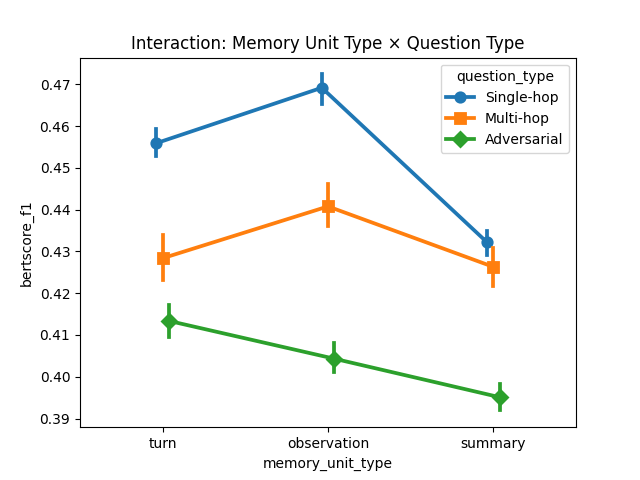
\includegraphics[width=0.75\textwidth]{charts/interaction_memory_unit_type_x_question_type.png}
\caption{Interactions between Memory Unit Type and Question Type}
\label{fig:interaction_memory_unit_type_x_question_type}
\end{figure}

% Plot
\begin{figure}[htbp]
\centering
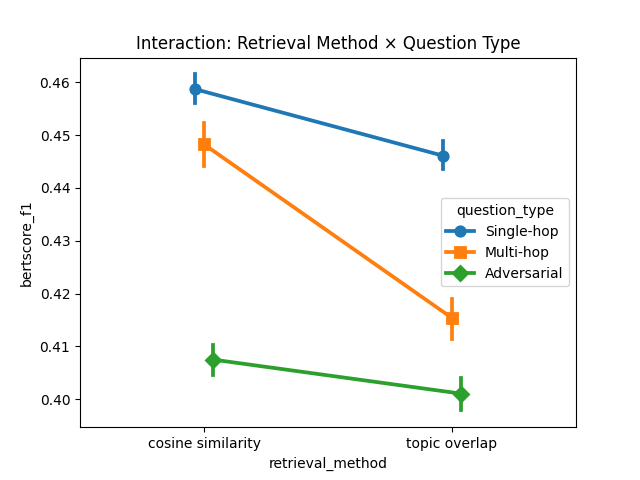
\includegraphics[width=0.75\textwidth]{charts/interaction_retrieval_method_x_question_type.png}
\caption{Interactions between Retrieval Method and Question Type}
\label{fig:interaction_retrieval_method_x_question_type}
\end{figure}

% Plot
\vspace*{0cm}
\begin{figure}[H]
\centering
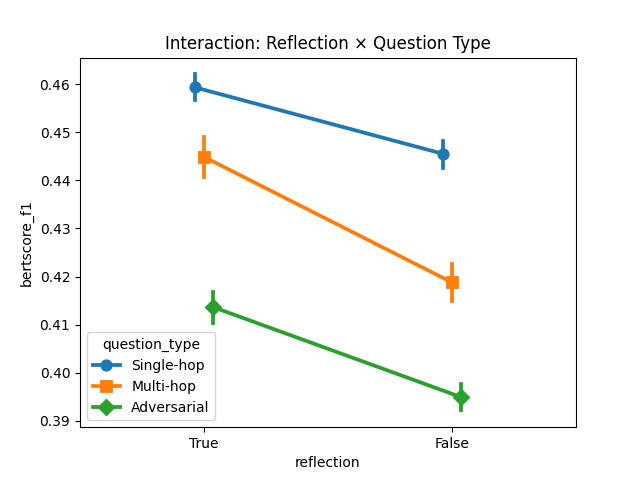
\includegraphics[width=0.75\textwidth]{charts/interaction_reflection_x_question_type.png}
\caption{Interactions between Reflection and Question Type}
\label{fig:interaction_reflection_x_question_type}
\end{figure}

\clearpage
